\subsection{Package \lstinline!cryptocast.client.filechooser!}
A generic implementation of a file chooser for Android applications.

\noindent\begin{minipage}[t]{5cm}
\vspace{0.3em}
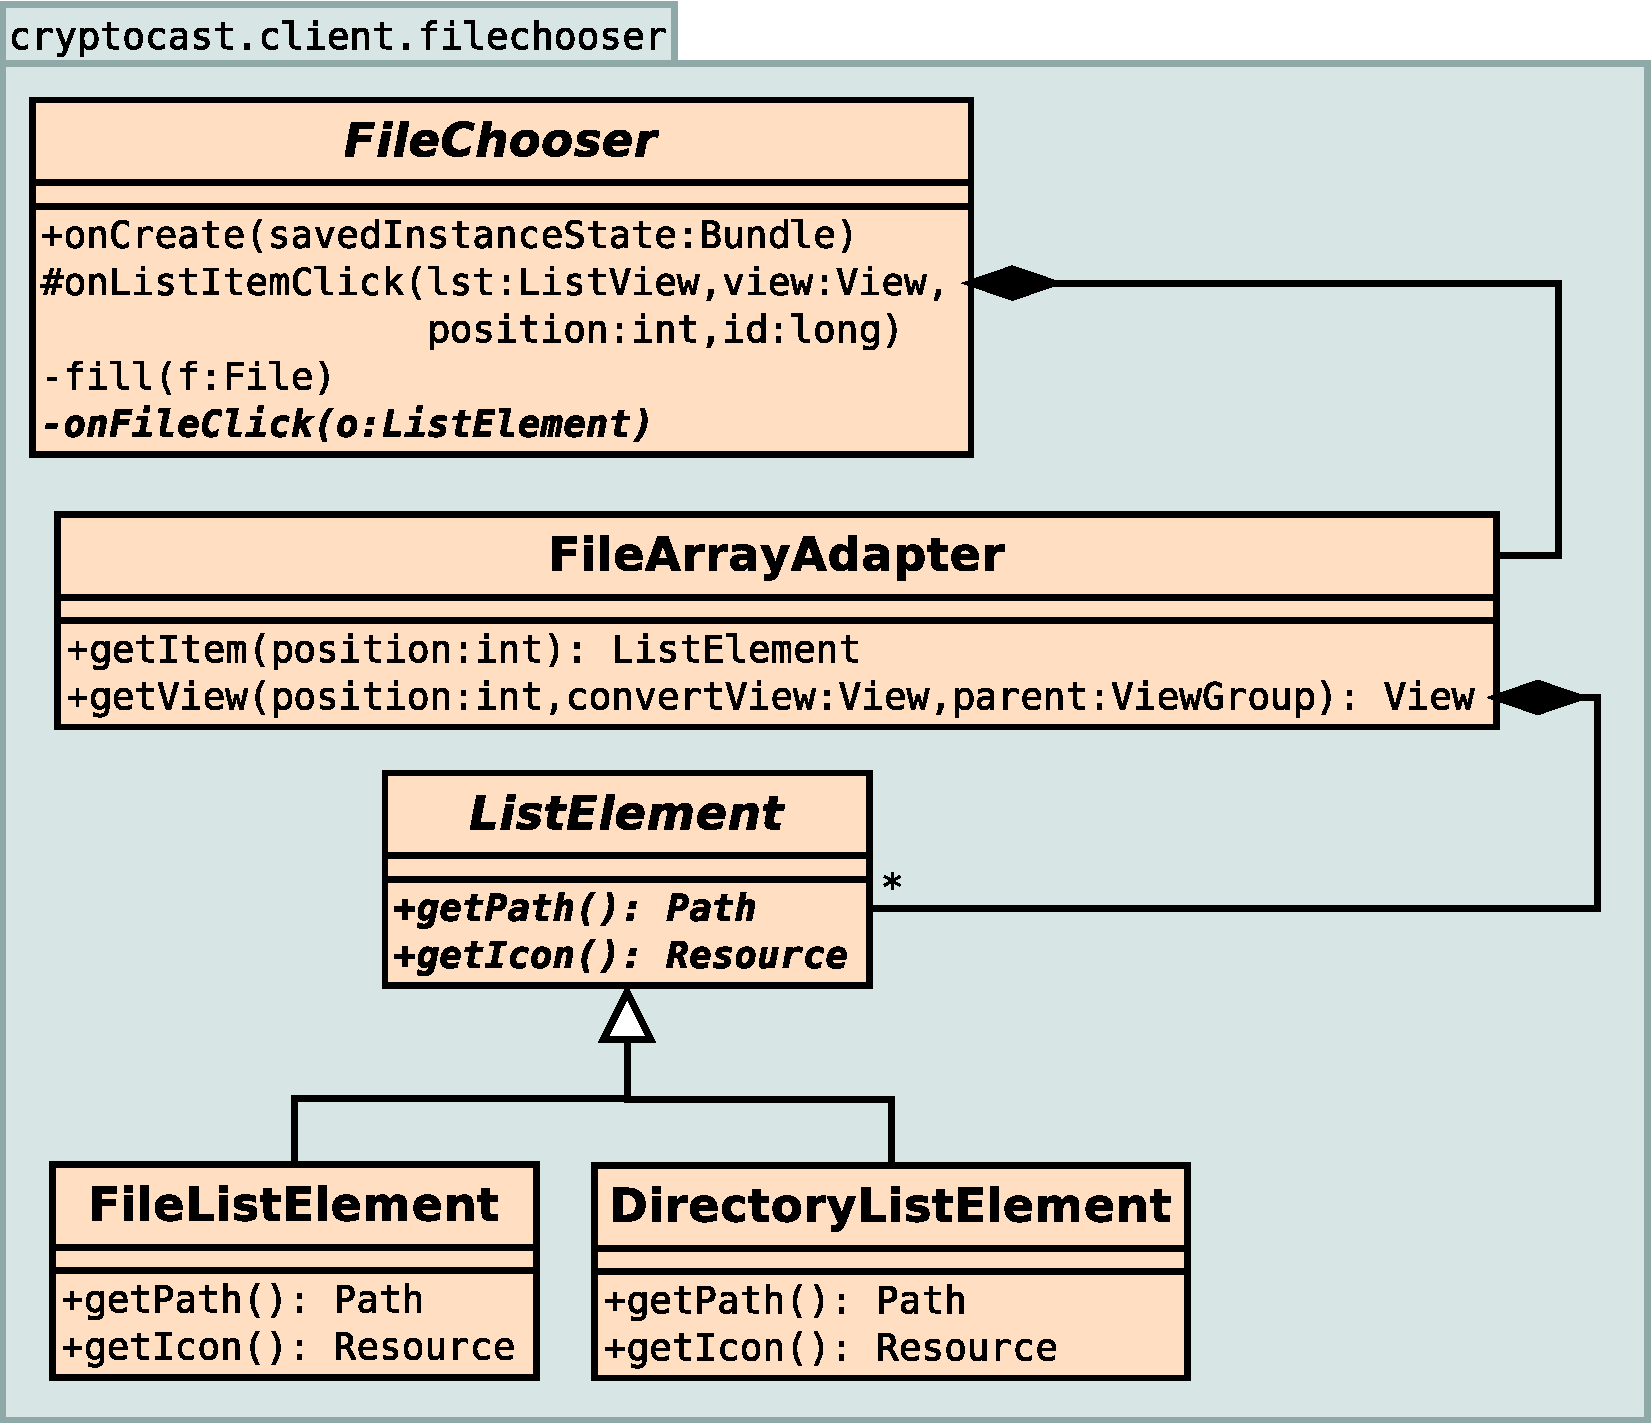
\includegraphics[width=300px]{class_diagrams/cryptocast_client_filechooser.pdf}
\end{minipage}

\subsubsection{Class \lstinline|ElementComparator|}
A comparator for ListElements based on their type id. \\
\noindent\begin{minipage}[t]{5cm}
\vspace{0.3em}
\hspace*{2em}
\begin{tikzpicture}
\umlclass[]{ElementComparator}{

}{
+ compare(e1 : ListElement, e2 : ListElement) : int
}
\end{tikzpicture}
\vspace{0.3em}
\end{minipage}



\textbf{\sffamily Superclasses and Interfaces}
\begin{itemize}
\item \lstinline|java.util.Comparator<ListElement>|
\end{itemize}



\textbf{\sffamily Methods}
\begin{itemize}
\item \lstinline|public int| \lstinline|compare|\lstinline|(ListElement e1, ListElement e2)| \\[-0.6em]




\end{itemize}

\subsubsection{Class \lstinline|NavigateUpListElement|}
A list element in our file chooser representing a directory. \\
\noindent\begin{minipage}[t]{5cm}
\vspace{0.3em}
\hspace*{2em}
\begin{tikzpicture}
\umlclass[]{NavigateUpListElement}{

}{
+ getPath() : File \\
+ getIcon(res : Resources) : Drawable \\
+ toString() : String \\
+ equals(other\_ : Object) : boolean
}
\end{tikzpicture}
\vspace{0.3em}
\end{minipage}



\textbf{\sffamily Superclasses and Interfaces}
\begin{itemize}
\item \lstinline|cryptocast.client.filechooser.ListElement|
\end{itemize}


\textbf{\sffamily Constructors}
\begin{itemize}
\item \lstinline|public| \lstinline|NavigateUpListElement|\lstinline|(File path)|\\ \\[-0.6em]
Creates a new instance.
\begin{itemize}
\item \lstinline|path|: The path of the directory
\end{itemize}



\end{itemize}


\textbf{\sffamily Methods}
\begin{itemize}
\item \lstinline|public File| \lstinline|getPath|\lstinline|()|\\ \\[-0.6em]
\emph{Returns:} The path of the element



\item \lstinline|public Drawable| \lstinline|getIcon|\lstinline|(Resources res)|\\ \\[-0.6em]
\emph{Returns:} The icon associated with this element.



\item \lstinline|public String| \lstinline|toString|\lstinline|()|\\ \\[-0.6em]
\emph{Returns:} A string representation of this element.



\item \lstinline|public boolean| \lstinline|equals|\lstinline|(Object other_)| \\[-0.6em]




\end{itemize}

\subsubsection{Class \lstinline|FileListElement|}
A list element in our file chooser, representing a file. \\
\noindent\begin{minipage}[t]{5cm}
\vspace{0.3em}
\hspace*{2em}
\begin{tikzpicture}
\umlclass[]{FileListElement}{

}{
+ getPath() : File \\
+ getIcon(res : Resources) : Drawable \\
+ toString() : String \\
+ equals(other\_ : Object) : boolean
}
\end{tikzpicture}
\vspace{0.3em}
\end{minipage}



\textbf{\sffamily Superclasses and Interfaces}
\begin{itemize}
\item \lstinline|cryptocast.client.filechooser.ListElement|
\end{itemize}


\textbf{\sffamily Constructors}
\begin{itemize}
\item \lstinline|public| \lstinline|FileListElement|\lstinline|(File path)|\\ \\[-0.6em]
Creates a new instance.
\begin{itemize}
\item \lstinline|path|: The path of the file
\end{itemize}



\end{itemize}


\textbf{\sffamily Methods}
\begin{itemize}
\item \lstinline|public File| \lstinline|getPath|\lstinline|()|\\ \\[-0.6em]
\emph{Returns:} The path of the element



\item \lstinline|public Drawable| \lstinline|getIcon|\lstinline|(Resources res)|\\ \\[-0.6em]
\emph{Returns:} The icon associated with this element.



\item \lstinline|public String| \lstinline|toString|\lstinline|()|\\ \\[-0.6em]
\emph{Returns:} A string representation of this element.



\item \lstinline|public boolean| \lstinline|equals|\lstinline|(Object other_)| \\[-0.6em]




\end{itemize}

\subsubsection{Class \lstinline|FileChooserState|}
Represents the state of a file chooser. \\
\noindent\begin{minipage}[t]{5cm}
\vspace{0.3em}
\hspace*{2em}
\begin{tikzpicture}
\umlclass[]{FileChooserState}{

}{
\umlstatic{+ fromDirectory(dir : File, filePattern : String) : FileChooserState} \\
\umlstatic{+ fromDirectory(dir : File) : FileChooserState} \\
\umlstatic{+ sortElements(list : List<ListElement>)} \\
+ getCurrentDir() : File \\
+ getItems() : ImmutableList<ListElement>
}
\end{tikzpicture}
\vspace{0.3em}
\end{minipage}




\textbf{\sffamily Constructors}
\begin{itemize}
\item \lstinline|private| \lstinline|FileChooserState|\lstinline|(File currentDir, ImmutableList<ListElement> items)| \\[-0.6em]




\end{itemize}


\textbf{\sffamily Methods}
\begin{itemize}
\item \lstinline|public static FileChooserState| \lstinline|fromDirectory|\lstinline|(File dir, String filePattern)|\\ \\[-0.6em]
Returns the state of the file chooser from the given directory and file pattern.
\begin{itemize}
\item \lstinline|dir|: The directory of the file.
\item \lstinline|filePattern|: The pattern of the file.
\end{itemize}

\emph{Returns:} the state of the file chooser from the given directory and file pattern.

\item \lstinline|public static FileChooserState| \lstinline|fromDirectory|\lstinline|(File dir)|\\ \\[-0.6em]
Returns the state of the file chooser from the given directory.
\begin{itemize}
\item \lstinline|dir|: The directory of the file.
\end{itemize}

\emph{Returns:} the state of the file chooser from the given directory.

\item \lstinline|public static void| \lstinline|sortElements|\lstinline|(List<ListElement> list)|\\ \\[-0.6em]
Sorts the given list.
\begin{itemize}
\item \lstinline|list|: The list to sort.
\end{itemize}



\item \lstinline|public File| \lstinline|getCurrentDir|\lstinline|()|\\ \\[-0.6em]
Returns the directory of the file.

\emph{Returns:} The directory of the file.

\item \lstinline|public ImmutableList<ListElement>| \lstinline|getItems|\lstinline|()| \\[-0.6em]




\end{itemize}

\subsubsection{Class \lstinline|FileArrayAdapter|}
An adapter between the ListElements and the view showing them. \\
\noindent\begin{minipage}[t]{5cm}
\vspace{0.3em}
\hspace*{2em}
\begin{tikzpicture}
\umlclass[]{FileArrayAdapter}{

}{
+ getView(position : int, convertView : View, parent : ViewGroup) : View
}
\end{tikzpicture}
\vspace{0.3em}
\end{minipage}



\textbf{\sffamily Superclasses and Interfaces}
\begin{itemize}
\item \lstinline|android.widget.ArrayAdapter<ListElement>|
\end{itemize}


\textbf{\sffamily Constructors}
\begin{itemize}
\item \lstinline|public| \lstinline|FileArrayAdapter|\lstinline|(Context context, Resources res, List<ListElement> elements)|\\ \\[-0.6em]
Constructs a new instance with the given attributes.
\begin{itemize}
\item \lstinline|context|: The context in which this adapter is used.
\end{itemize}



\end{itemize}


\textbf{\sffamily Methods}
\begin{itemize}
\item \lstinline|public View| \lstinline|getView|\lstinline|(int position, View convertView, ViewGroup parent)|\\ \\[-0.6em]
\emph{Returns:} A custom view of a list element at the given position in the list.
\begin{itemize}
\item \lstinline|position|: The position of the element in the list
\item \lstinline|convertView|: View which should be converted
\item \lstinline|parent|: The parent view group
\end{itemize}



\end{itemize}

\subsubsection{Class \lstinline|FileChooser|}
A file chooser that is used to choose a key file from the filesystem. \\
\noindent\begin{minipage}[t]{5cm}
\vspace{0.3em}
\hspace*{2em}
\begin{tikzpicture}
\umlclass[]{FileChooser}{

}{
+ getFilePattern() : String \\
+ init(act : Activity) \\
+ onItemClick(arg0 : AdapterView<?>, arg1 : View, pos : int, arg3 : long)
}
\end{tikzpicture}
\vspace{0.3em}
\end{minipage}



\textbf{\sffamily Superclasses and Interfaces}
\begin{itemize}
\item \lstinline|android.widget.AdapterView.OnItemClickListener|
\end{itemize}


\textbf{\sffamily Constructors}
\begin{itemize}
\item \lstinline|public| \lstinline|FileChooser|\lstinline|(String filePattern)|\\ \\[-0.6em]
Initializes a file with the given file pattern.
\begin{itemize}
\item \lstinline|filePattern|: The pattern of the file.
\end{itemize}



\end{itemize}


\textbf{\sffamily Methods}
\begin{itemize}
\item \lstinline|public String| \lstinline|getFilePattern|\lstinline|()|\\ \\[-0.6em]
Returns the pattern of the file.

\emph{Returns:} The pattern of the file.

\item \lstinline|public void| \lstinline|init|\lstinline|(Activity act)|\\ \\[-0.6em]
initializes the file chooser for the given activity.
\begin{itemize}
\item \lstinline|act|: The activity.
\end{itemize}



\item \lstinline|public void| \lstinline|onItemClick|\lstinline|(AdapterView<?> arg0, View arg1, int pos, long arg3)| \\[-0.6em]




\end{itemize}

\subsubsection{Class \lstinline|DirectoryListElement|}
A list element in our file chooser representing a directory. \\
\noindent\begin{minipage}[t]{5cm}
\vspace{0.3em}
\hspace*{2em}
\begin{tikzpicture}
\umlclass[]{DirectoryListElement}{

}{
+ getPath() : File \\
+ getIcon(res : Resources) : Drawable \\
+ toString() : String \\
+ equals(other\_ : Object) : boolean
}
\end{tikzpicture}
\vspace{0.3em}
\end{minipage}



\textbf{\sffamily Superclasses and Interfaces}
\begin{itemize}
\item \lstinline|cryptocast.client.filechooser.ListElement|
\end{itemize}


\textbf{\sffamily Constructors}
\begin{itemize}
\item \lstinline|public| \lstinline|DirectoryListElement|\lstinline|(File path)|\\ \\[-0.6em]
Creates a new instance.
\begin{itemize}
\item \lstinline|path|: The path of the directory
\end{itemize}



\end{itemize}


\textbf{\sffamily Methods}
\begin{itemize}
\item \lstinline|public File| \lstinline|getPath|\lstinline|()|\\ \\[-0.6em]
\emph{Returns:} The path of the element



\item \lstinline|public Drawable| \lstinline|getIcon|\lstinline|(Resources res)|\\ \\[-0.6em]
\emph{Returns:} The icon associated with this element.



\item \lstinline|public String| \lstinline|toString|\lstinline|()|\\ \\[-0.6em]
\emph{Returns:} A string representation of this element.



\item \lstinline|public boolean| \lstinline|equals|\lstinline|(Object other_)| \\[-0.6em]




\end{itemize}

\subsubsection{Interface \lstinline|ListElement|}
A list element in our file chooser, representing an element on the file system. \\
\noindent\begin{minipage}[t]{5cm}
\vspace{0.3em}
\hspace*{2em}
\begin{tikzpicture}
\umlclass[type=abstract]{ListElement}{

}{
\umlvirt{+ getPath() : File} \\
\umlvirt{+ getIcon(res : Resources) : Drawable}
}
\end{tikzpicture}
\vspace{0.3em}
\end{minipage}





\textbf{\sffamily Methods}
\begin{itemize}
\item \lstinline|public File| \lstinline|getPath|\lstinline|()|\\ \\[-0.6em]
\emph{Returns:} The path of the element



\item \lstinline|public Drawable| \lstinline|getIcon|\lstinline|(Resources res)|\\ \\[-0.6em]
\emph{Returns:} The icon associated with this element.



\end{itemize}


